\documentclass[
  bibliography=totoc,     % Literatur im Inhaltsverzeichnis
  captions=tableheading,  % Tabellenüberschriften
  titlepage=firstiscover, % Titelseite ist Deckblatt
]{scrartcl}

% Paket float verbessern
\usepackage{scrhack}

% Warnung, falls nochmal kompiliert werden muss
\usepackage[aux]{rerunfilecheck}

% unverzichtbare Mathe-Befehle
\usepackage{amsmath}
% viele Mathe-Symbole
\usepackage{amssymb}
% Erweiterungen für amsmath
\usepackage{mathtools}

% Fonteinstellungen
\usepackage{fontspec}
% Latin Modern Fonts werden automatisch geladen
% Alternativ zum Beispiel:
%\setromanfont{Libertinus Serif}
%\setsansfont{Libertinus Sans}
%\setmonofont{Libertinus Mono}

% Wenn man andere Schriftarten gesetzt hat,
% sollte man das Seiten-Layout neu berechnen lassen
\recalctypearea{}

% deutsche Spracheinstellungen
\usepackage[ngerman]{babel}


\usepackage[
  math-style=ISO,    % ┐
  bold-style=ISO,    % │
  sans-style=italic, % │ ISO-Standard folgen
  nabla=upright,     % │
  partial=upright,   % │
  mathrm=sym,        % ┘
  warnings-off={           % ┐
    mathtools-colon,       % │ unnötige Warnungen ausschalten
    mathtools-overbracket, % │
  },                       % ┘
]{unicode-math}

% traditionelle Fonts für Mathematik
\setmathfont{Latin Modern Math}
% Alternativ zum Beispiel:
%\setmathfont{Libertinus Math}

\setmathfont{XITS Math}[range={scr, bfscr}]
\setmathfont{XITS Math}[range={cal, bfcal}, StylisticSet=1]

% Zahlen und Einheiten
\usepackage[
  locale=DE,                   % deutsche Einstellungen
  separate-uncertainty=true,   % immer Unsicherheit mit \pm
  per-mode=symbol-or-fraction, % / in inline math, fraction in display math
]{siunitx}

% chemische Formeln
\usepackage[
  version=4,
  math-greek=default, % ┐ mit unicode-math zusammenarbeiten
  text-greek=default, % ┘
]{mhchem}

% richtige Anführungszeichen
\usepackage[autostyle]{csquotes}

% schöne Brüche im Text
\usepackage{xfrac}

% Standardplatzierung für Floats einstellen
\usepackage{float}
\floatplacement{figure}{htbp}
\floatplacement{table}{htbp}

% Floats innerhalb einer Section halten
\usepackage[
  section, % Floats innerhalb der Section halten
  below,   % unterhalb der Section aber auf der selben Seite ist ok
]{placeins}

% Seite drehen für breite Tabellen: landscape Umgebung
\usepackage{pdflscape}

% Captions schöner machen.
\usepackage[
  labelfont=bf,        % Tabelle x: Abbildung y: ist jetzt fett
  font=small,          % Schrift etwas kleiner als Dokument
  width=0.9\textwidth, % maximale Breite einer Caption schmaler
]{caption}
% subfigure, subtable, subref
\usepackage{subcaption}

% Grafiken können eingebunden werden
\usepackage{graphicx}

% schöne Tabellen
\usepackage{tabularray}
\UseTblrLibrary{booktabs, siunitx}

% Verbesserungen am Schriftbild
\usepackage{microtype}

% Literaturverzeichnis
\usepackage[
  backend=biber,
]{biblatex}
% Quellendatenbank
\addbibresource{lit.bib}
\addbibresource{programme.bib}

% Hyperlinks im Dokument
\usepackage[
  german,
  unicode,        % Unicode in PDF-Attributen erlauben
  pdfusetitle,    % Titel, Autoren und Datum als PDF-Attribute
  pdfcreator={},  % ┐ PDF-Attribute säubern
  pdfproducer={}, % ┘
]{hyperref}
% erweiterte Bookmarks im PDF
\usepackage{bookmark}

% Trennung von Wörtern mit Strichen
\usepackage[shortcuts]{extdash}

\author{%
  Vincent Wirsdörfer\\%
  \href{mailto:vincent.wirsdoerfer@udo.edu}{authorA@udo.edu}%
  \and%
  Joris Daus\\%
  \href{mailto:joris.daus@udo.edu}{authorB@udo.edu}%
}
\publishers{TU Dortmund – Fakultät Physik}


\begin{document}
\section{Versuchsaufbau}

\noindent Aufgrund der Tatsache, dass in diesem Versuch verschiedene Methoden zur Bestimmung derselben physikalischen Größe 
durchgeführt werden, wird der Versuchsaufbau des Öfteren leicht variiert. Dessen ungeachtet beruhen alle Methoden auf 
einem grundsätzlichen Konstrukt, welches im Folgenden näher erläutert wird. Der allgemeine Versuchsaufbau wird in der 
Abbildung dargestellt.

\begin{figure}[H]
    \centering
    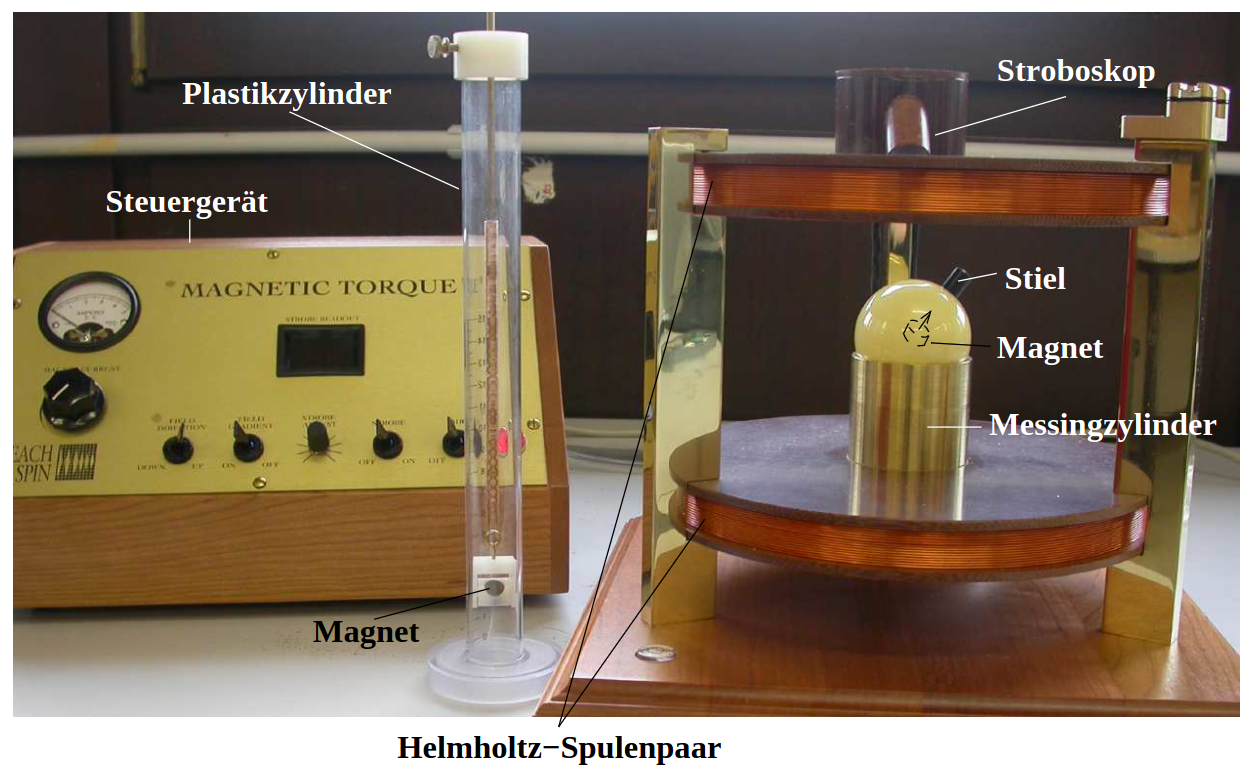
\includegraphics[height=6cm]{aufbau.png}
    \caption{Versuchsaufbau zur Bestimmung des magnetischen Momentes \cite{Versuchsanleitung_v105}.}
    \label{fig:aufbau_moment}
\end{figure}

\noindent Wie in der Grafik \ref{fig:aufbau_moment} gezeigt, befindet sich ein zylindrischer Permanentmagnet in der Mitten einer 
kugelförmigen Billardkugel. Diese Billardkugel wird auf einen Messingzylinder gesetzt und kann durch ein integriertes Luftkissen
in Bewegung versetzt werden. Zusätzlich ragt aus der Billardkugel ein Stiel heraus, welcher zusätzlich mit einer schmalen 
Aluminiumstange durchstoßen werden kann. An dieser Stangen ebenfalls eine Masse befestigt werden. Diese Erweiterung des Aufbaus 
ist jedoch nur bei der Gravitations-Methode von Bedeutung.\\
Umgeben ist der Permanentmagnet von einem Helmholtz-Spulenpaar mit einer Windungszahl von $N = 195$ und einem Spulenabstand 
$d = 0.138\,\unit{\meter}$. Der Spulenradius liegt bei $R_\text{Spule} = 0.109\,\unit{\meter}$. An der oberen Spule ist 
ein Stroboskop angebracht, welches die Kreisfrequenz der Billardkugel bei der Präzessions-Methode regelt.\\
Konkret angepasst wird der Spulenstrom, die Feldrichtung, der Feldgradient und die Frequenz des Stroboskops durch, das in der 
Abbildung links stehende Steuergerät.


\section{Versuchsdurchführung}
\subsection{Präzessions-Methode}

\noindent Bei der ersten Methode soll das magnetische Moment des über die Präzession des Permanentmagneten im homogenen 
B-Feld des Helmholtz-Spulenpaars bestimmt werden. Dazu werden zunächst einige Testläufe bei ausgeschaltetem Spulenstrom 
durchgeführt, um sich mit dem Rotationsverhalten der Billardkugel vertraut zu machen. Im Anschluss wird versucht die Kreisfrequenz 
der rotierenden Kugel mit der Frequenz der Lichtblitze des Stroboskops in Einklang zu bringen. Um dies zu verifizieren, wird 
die Versuchsapparatur mittels einer Jacke dienend als \enquote{Vorhang} abgedunkelt, um die Lichtblitze auf dem Stiel besser 
erkennen zu können. Ist dies geschafft, wird der tatsächliche Versuch eingeleitet. Zunächst wird das Stroboskop auf eine 
Frequenz von $f = 5.5\,\unit{\hertz}$ eingestellt. Dann wird die Billardkugel in Rotation versetzt und mittels leichter
Berührungen eines Stabes von Nutationsbewegungen befreit und auf die Frequenz des Stroboskop gebracht. Erscheint der Punkt auf 
der Oberfläche des Stiels als stationär, sind die Frequenzen nahezu identisch. An diesem Punkt wird nun der Spulenstrom 
eingeschaltet, um ein magnetisches Feld zu erzeugen. Diese äußere Kraft bewirkt nun eine Präzessionsbewegung der Kugel. Es wird 
die Zeit $T_\text{P}$ für einen Umlauf des Stiels gemessen. Für eine Stromstärke werden drei Messungen durchgeführt. Insgesamt werden 
die Umlaufzeiten von fünf Stromstärken aufgenommen, was total 15 Messungen ergibt. Zwischen den Messungen wird der Spulenstrom 
abgeschaltet, um Überhitzungen und fortwährende Präzessionsbewegungen zu vermeiden.

\subsection{Gravitations-Methode}

\noindent Zu Beginn der Gravitations-Methode werden essenzielle geometrische Abmessungen gemacht, um das Dipolmoment des 
Permanentmagneten durch Gleichsetzen der Drehmomente ermitteln zu können. Im Anschluss wird eine bestimmte Abmessung $r_1$ 
an der Aluminiumstange durchgeführt. Zusammen mit der angebrachten Masse wird der Aluminiumstab in den Stiel der Kugel gesteckt. 
Am Steuergerät wird nun das Gebläse des Luftkissens eingeschaltet, die Feldrichtung auf \enquote{up} und der Feldgradient auf 
\enquote{off} eingestellt. Um ein einheitliches Gleichgewicht bei allen Versuchen festzulegen wird die Aluminiumstange zunächst auf 
dem Spulenrand abgelegt. Im Folgenden wird das B-Feld so reguliert, dass der Stab leicht abhebt und sich ohne zusätzliche 
Abstoßung am Spulenrand im Magnetfeld befindet. Dann ist ein Gleichgewicht erreicht. Wegen sich wiederholenden Aussetzern des 
Luftkissens, wird die Kugel oft leicht berührt, um den Kontakt zwischen Luftkissen und Kugel gewährleisten zu können.
Nach Erreichen des Gleichgewichts und Notation des dafür notwendigen Spulenstroms, wird der Stab entfernt und eine neue Abmessung 
$r_2$ vorgenommen. Die Versuchsdurchführung wird wiederholt und bis zu einer Abmessung $r_10$ vollzogen. Auch hier wird der 
Spulenstrom zwischen den einzelnen Durchführungen abgeschaltet.

\subsection{Schwingungs-Methode}

\noindent Bei der letzten Methode wird das magnetische Moment über die Schwingungsdauer der Billardkugel ermittelt. Hierbei wird
die Kugel auf das Luftkissen gesetzt und das B-Feld durch den Spulenstrom eingeschaltet. Nun wird die Kugel um einen kleinen Winkel 
ausgelenkt und durch das eingeschaltete Magnetfeld in Schwingung versetzt. Es wird genau die Zeit gemessen und notiert, welche 
die Kugel für zehn Periodendauern benötigt. Dieser Versuch wird für neun weiter Stromstärken wiederholt.

\section{Messwerte}

\end{document}

